\documentclass[border=3pt]{standalone}
%\usepackage{amsthm}
\usepackage{amsmath}
\usepackage{amssymb}
\usepackage{natbib}
\usepackage[colorlinks,citecolor=blue,urlcolor=blue,filecolor=blue,backref=page]{hyperref}
\usepackage{graphicx}
\usepackage{subfigure}
\usepackage{bm}
\usepackage{booktabs}
\usepackage{listings}
\usepackage{color}

\usepackage{tikz}
\usetikzlibrary{shapes.misc}
\usetikzlibrary{matrix}
\usetikzlibrary{arrows,backgrounds,fit,calc,shapes,automata}
\usetikzlibrary{bayesnet}
\tikzstyle{every picture}+=[remember picture]
\tikzset{
    %Define standard arrow tip
    >=stealth',
    %Define style for boxes¡
    punkt/.style={
           rectangle,
           rounded corners,
           draw=black,
           thick,
           text width=3.5cm,
           minimum height=1.0cm,
           text centered},
    % Define arrow style
    pil/.style={
           ->,
           thick,
           shorten <=2pt,
           shorten >=2pt,}
}
\usetikzlibrary{decorations.pathreplacing,shapes}
\pagestyle{empty}

\begin{document}
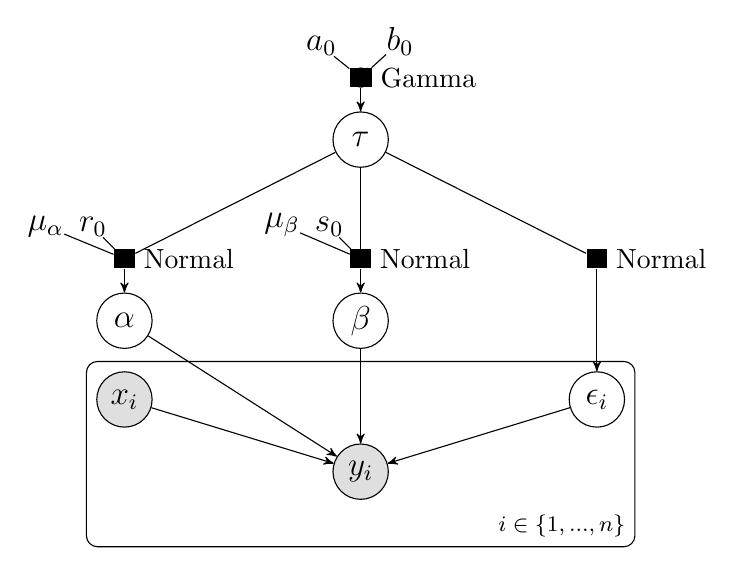
\begin{tikzpicture}[scale=1.0, transform shape]
  [squarednode/.style={rectangle, draw=black, minimum size=8mm},
    latent/.style={circle, draw=black, minimum size=10mm}]

  % \footnotesize

  % Define nodes
  \node[obs] (y) {\large $y_i$};

  \node[obs, above=0.2cm of y, xshift=-3.0cm] (x) {\large $x_i$};


  \node[latent, above=0.2cm of y, xshift=3.0cm]  (epsilon) {\large $\epsilon_i$};



  \node[latent, above=3.5cm of y, xshift=0cm]  (tau) {\large $\tau$};
  \node[factor, above=0.3cm of tau, xshift=0cm]  (G1) {G};
  \node[const, right=0.1cm of G1] () {\normalsize Gamma};
  \node[const, above=0.7cm of tau, xshift=-0.5cm] (a0) {\large $a_0$};
  \node[const, above=0.7cm of tau, xshift=0.5cm] (b0) {\large $b_0$};

  \node[latent, above=1.2cm of y, xshift=-3.0cm]  (alpha) {\large $\alpha$};
  \node[factor, above=0.3cm of alpha, xshift=0cm]  (N2) {N};
  \node[const, right=0.1cm of N2] () {\normalsize Normal};
  \node[const, above=0.7cm of alpha, xshift=-1.0cm] (mu_alpha) {\large $\mu_\alpha$};
  \node[const, above=0.7cm of alpha, xshift=-0.4cm] (r0) {\large $r_0$};

  \node[latent, above=1.2cm of y, xshift=0.0cm]  (beta) {\large $\beta$};
  \node[factor, above=0.3cm of beta, xshift=0cm]  (N3) {N};
  \node[const, right=0.1cm of N3] () {\normalsize Normal};
  \node[const, above=0.7cm of beta, xshift=-1.0cm] (mu_beta) {\large $\mu_\beta$};
  \node[const, above=0.7cm of beta, xshift=-0.4cm] (s0) {\large $s_0$};


  \node[factor, above=0.3cm of beta, xshift=3.0cm]  (N1) {N};
  \node[const, right=0.1cm of N1] () {\normalsize Normal};

  \draw [->] (x) -- (y);
  \draw [->] (alpha) -- (y);
  \draw [->] (beta) -- (y);
  \draw [->] (epsilon) -- (y);

  \factoredge{tau}{N1}{epsilon};
  \factoredge{tau,mu_alpha,r0}{N2}{alpha};
  \factoredge{tau,mu_beta,s0}{N3}{beta};
  \factoredge{a0,b0}{G1}{tau};

  \plate {} {(y)(x)(epsilon)} {$i \in \lbrace 1, ..., n \rbrace$}; %

\end{tikzpicture}
\end{document}
